%%%%%%%%%%%%%%%%%%%%%%%%%%%%%%%%%%%%%%%%%
% University/School Laboratory Report
% LaTeX Template
% Version 3.1 (25/3/14)
%
% This template has been downloaded from:
% http://www.LaTeXTemplates.com
%
% Original author:
% Linux and Unix Users Group at Virginia Tech Wiki 
% (https://vtluug.org/wiki/Example_LaTeX_chem_lab_report)
%
% License:
% CC BY-NC-SA 3.0 (http://creativecommons.org/licenses/by-nc-sa/3.0/)
%
%%%%%%%%%%%%%%%%%%%%%%%%%%%%%%%%%%%%%%%%%

%----------------------------------------------------------------------------------------
%	PACKAGES AND DOCUMENT CONFIGURATIONS
%----------------------------------------------------------------------------------------

\documentclass{article}

\usepackage{xeCJK}
\usepackage[version=3]{mhchem} % Package for chemical equation typesetting
\usepackage{siunitx} % Provides the \SI{}{} and \si{} command for typesetting SI units
\usepackage{graphicx} % Required for the inclusion of images
\usepackage{natbib} % Required to change bibliography style to APA
\usepackage{amsmath} % Required for some math elements 

\setlength\parindent{0pt} % Removes all indentation from paragraphs

\renewcommand{\labelenumi}{\alph{enumi}.} % Make numbering in the enumerate environment by letter rather than number (e.g. section 6)

%\usepackage{times} % Uncomment to use the Times New Roman font
\usepackage{float}
\usepackage{amsmath}
\usepackage{listings}
\usepackage{color}

\definecolor{dkgreen}{rgb}{0,0.6,0}
\definecolor{gray}{rgb}{0.5,0.5,0.5}
\definecolor{mauve}{rgb}{0.58,0,0.82}

\lstset{frame=tb,
  language=C++,
  aboveskip=3mm,
  belowskip=3mm,
  showstringspaces=false,
  columns=flexible,
  basicstyle={\small\ttfamily},
  numbers=none,
  numberstyle=\tiny\color{gray},
  keywordstyle=\color{blue},
  commentstyle=\color{dkgreen},
  stringstyle=\color{mauve},
  breaklines=true,
  breakatwhitespace=true,
  tabsize=3
}



%----------------------------------------------------------------------------------------
%	DOCUMENT INFORMATION
%----------------------------------------------------------------------------------------

\title{柱面全景拼接Panorama实现 \\ 计算摄影学} % Title

\author{杨晗 \\ 3150104251} % Author name

\date{\today} % Date for the report

\begin{document}

\maketitle % Insert the title, author and date

\begin{center}
\begin{tabular}{l r}
\end{tabular}
\end{center}


% If you wish to include an abstract, uncomment the lines below
% \begin{abstract}
% Abstract text
% \end{abstract}

%----------------------------------------------------------------------------------------
%	SECTION 1
%----------------------------------------------------------------------------------------

\section{背景}

全景图拼接是利用同一场景的多张图像通过重叠部分寻找匹配关系,从而生成整个场景图像的技术。 全景图的拼接方法有很多,如按场景和运动的种类可以分为单视点全景拼接和多视点全景拼接。对于平面场景和只通过相机旋转拍摄的场景来说,可以使用求每两幅图像之间的一个Homography变换来映射到一张图像的方法,还可以使用恢复相机的旋转的方式得到最终的全景图。当相机固定只有水平方向旋转时,也可以使用柱面或球面坐标映射的方式求得全景图。
% \begin{center}\ce{2 Mg + O2 -> 2 MgO}\end{center}

% If you have more than one objective, uncomment the below:
%\begin{description}
%\item[First Objective] \hfill \\
%Objective 1 text
%\item[Second Objective] \hfill \\
%Objective 2 text
%\end{description}

\section{实验目标}
实现一个Panorama类,实现给定一组序列图片和焦距,输出拼接的全景图像的功能。
% \label{definitions}
% \begin{description}
% \item[Stoichiometry]
% The relationship between the relative quantities of substances taking part in a reaction or forming a compound, typically a ratio of whole integers.
% \item[Atomic mass]
% The mass of an atom of a chemical element expressed in atomic mass units. It is approximately equivalent to the number of protons and neutrons in the atom (the mass number) or to the average number allowing for the relative abundances of different isotopes. 
% \end{description} 
 
%----------------------------------------------------------------------------------------
%	SECTION 2
%----------------------------------------------------------------------------------------

\section{实验环境}
% \label{definitions}
\begin{description}
\item[Windows 10, i5-4210H]
\item[OpenCV 3.3]
\end{description}
\subsection{补充}
OpenCV 3 与 OpenCV 2 相比,提取特征的接口发生了较大变化,SIFT等特征提取的代码被移到contrib的xfeatures2d中。此为编译运行需要注意的点。

\section{算法原理}

% \begin{tabular}{ll}
% Mass of empty crucible & \SI{7.28}{\gram}\\
% Mass of crucible and magnesium before heating & \SI{8.59}{\gram}\\
% Mass of crucible and magnesium oxide after heating & \SI{9.46}{\gram}\\
% Balance used & \#4\\
% Magnesium from sample bottle & \#1
% \end{tabular}
\subsection{柱面投影}
\subsubsection{目标}
把平面图像投影到柱面上。
\subsubsection{原理}

\begin{equation}
x^{'}=f*atan\left(\frac {x-0.5*width}{f}\right)+f*atan\left( \frac {0.5*width}{f}\right)
\end{equation}
\begin{equation}
y^{'}=\frac {f*(y-0.5*height)}{\sqrt {(x-0.5*width)^2+f^2}}+0.5*height
\end{equation}
\begin{figure}[H]
\begin{center}
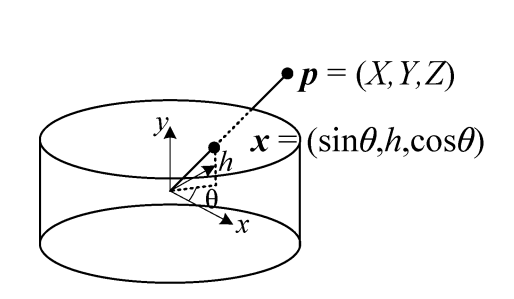
\includegraphics[width=0.65\textwidth]{transform} % Include the image placeholder.png
\caption{柱面投影变换}
\end{center}
\end{figure}


\subsection{特征抽取与匹配}
\subsubsection{目标}
对每两幅相邻的柱面图像进行特征提取和匹配,寻找两幅相邻图像的对应关系。
\subsubsection{原理}
SIFT 特征是基于物体上的一些局部外观的兴趣点而与影像的大小和旋转无关。对于光线、噪声、些微视角改变的容忍度也相当高。\\
通过SIFT特征的提取,然后用BruteForceMatch或者KnnMatch可以对SIFT计算出匹配。
用匹配的特征点可以训练出homography。
\subsection{计算变换,进行拼接}
\subsubsection{目标}
使用得到的匹配关系,求出每两幅柱面图像的平移变换,利用平移变换将所有图像拼接到一起。得到全景图。
\subsubsection{原理}
通过RANSAC之后的匹配特征点,可以从中计算得出homography。利用这个homography,可以算出图片的变换,利用此变换可以将两幅图像拼接在一起。
%----------------------------------------------------------------------------------------
%	SECTION 3
%----------------------------------------------------------------------------------------

\section{代码实现}
\subsection{接口}
核心代码是实现如下的接口:
\begin{lstlisting}
class CylindricalPanorama
{
public:
    virtual bool makePanorama(
        std::vector<cv::Mat>& img_vec, cv::Mat& img_out, double f
    ) = 0;
};
\end{lstlisting}
我实现的类如下:
\begin{lstlisting}
class Panorama4251 : public CylindricalPanorama {
    public:
        Panorama4251();
        ~Panorama4251();
        bool makePanorama(vector<Mat>& img_vec, Mat& img_out, double f);
    private:
        Mat cylinder(Mat& img, double f);
        Mat stitch(Mat& img, Mat& img1);
}
\end{lstlisting}
\subsection{代码流程}
我实现的流程如下:
\begin{enumerate}  
    \item 对列表中所有图片进行柱面投影,并存下来
    \item 对于上一次的拼接结果和下一张图片求SIFT特征点
    \item 匹配SIFT特征点
    \item 计算homography
    \item 利用homography进行变换,拼接
    \item 重复上述步骤直到用完所有图片,完成全景拼接
\end{enumerate}
这里有一个细节是如果从左往右拼接的话,最好是把左边的图片变换到右边图片的坐标系中,
这样可以方便之后的特征点匹配和homography的计算。
\subsection{柱面投影}
这里通过最近邻插值算法来求柱面图上的点到原图的对应位置,并用此位置的像素值作为此点的像素值。

\begin{lstlisting}
Mat cylinder(Mat& img, double f) {
    Mat output;
    int cols = (int)2 * f * atan(0.5*img.cols / f);
    int rows = (int)img.rows;
    output.create(rows, cols, CV_8UC3);
    for (int i = 0; i < rows; i++) {
        for (int j = 0; j < cols; j++) {
            int x = (int)(f * tan((float)(j - cols * 0.5) / f) + img.cols*0.5);
            int y = (int)((i - 0.5*rows)*sqrt(pow(x - img.cols*0.5, 2) + f*f) / f + 0.5*img.rows);
            if (0 <= x && x < img.cols && 0 <= y && y < img.rows) {
                output.at<Vec3b>(i, j) = img.at<Vec3b>(y, x);
            }
            else {
                output.at<Vec3b>(i, j) = Vec3b(0, 0, 0);
            }
        }
    }
    return output;
}
\end{lstlisting}
\subsubsection{特征点提取}
这里的SIFT特征点是用OpenCV 3 的写法。
\begin{lstlisting}
    Ptr<Feature2D> f2d = xfeatures2d::SIFT::create();
    vector<KeyPoint> kps_0, kps_1;
    f2d->detect(img_1, kps_0);
    f2d->detect(img_2, kps_1);

    Mat descriptors_0, descriptors_1;
    f2d->compute(img_1, kps_0, descriptors_0);
    f2d->compute(img_2, kps_1, descriptors_1);
\end{lstlisting}
\subsubsection{特征点的匹配和筛选}
其中对于distance过大的点进行了筛选处理,保留比较好的点。
\begin{lstlisting}
    FlannBasedMatcher matcher;
    //BFMatcher matcher;
    vector<DMatch> matches;
    matcher.match(descriptors_0, descriptors_1, matches);
    sort(matches.begin(), matches.end());
    float min_v = numeric_limits<float>::max();
    float max_v = 0;
    for (int i = 0; i < matches.size(); ++i) {
        min_v = min(min_v, matches[i].distance);
        max_v = max(max_v, matches[i].distance);
    }
    vector<Point2f> ps_0, ps_1;
    //assert(matches.size() > 500);
    cout << "min_v " << min_v << endl;
    cout << "max_v " << max_v << endl;
    for (int i = 0; i<matches.size(); ++i) {
        DMatch m = matches[i];
        if (m.distance > max_v / 2 )continue;
        ps_0.push_back(kps_0[m.queryIdx].pt);
        ps_1.push_back(kps_1[m.trainIdx].pt);
    }
\end{lstlisting}
\subsubsection{计算homography并计算图像扩大行列}
利用匹配点来计算出Homography。\\
并且利用边界点计算出拼接后的图像的大小。
\begin{lstlisting}			
    Mat rev_H = findHomography(ps_1, ps_0, RANSAC);
    Mat H = findHomography(ps_0, ps_1, RANSAC);

    cout << "begin stitcher....  " << i << endl;
    vector<Point2f> corners_1(4);
    vector<Point2f> corners_2(4);
    corners_1[0] = Point2f(0, 0);
    corners_1[1] = Point2f((float)img_1.cols, 0);
    corners_1[2] = Point2f((float)img_1.cols, (float)img_1.rows);
    corners_1[3] = Point2f(0, (float)img_1.rows);

    perspectiveTransform(corners_1, corners_2, H);
    int down_rows = (int)min(corners_2[0].y, corners_2[1].y);
    down_rows = min(0, down_rows) * -1;
    int right_cols = (int)min(corners_2[0].x, corners_2[3].x);
    right_cols = min(0, right_cols) * -1;
\end{lstlisting}
\subsubsection{计算变换后的坐标并进行变换,拼接}
这里计算了每个点在新坐标系下的位置,并进行了插值。
\begin{lstlisting}
    Mat stitch_img = Mat::zeros(img_2.rows+down_rows, img_2.cols+right_cols, CV_8UC3);
    img_2.copyTo(Mat(stitch_img, Rect(right_cols, down_rows, img_2.cols, img_2.rows)));
    for (int i = 0; i < stitch_img.rows; ++i) {
        for (int j = 0; j < stitch_img.cols; ++j) {
            if (stitch_img.at<Vec3b>(i, j) != Vec3b(0, 0, 0)) {
                continue;
            }
            int x0 = j - right_cols;
            int y0 = i - down_rows;
            vector<Point2f> pix, dst;
            pix.emplace_back(x0, y0);
            perspectiveTransform(pix, dst, rev_H);
            Point2f pos = dst[0];
            //cout << pos << endl;
            int x = (int)floor(pos.x);
            int y = (int)floor(pos.y);
            if (0 < y && y < img_1.rows && 0 < x && x < img_1.cols && img_1.at<Vec3b>(y,x) != Vec3b(0,0,0) ) {
                Vec3b c = img_1.at<Vec3b>(y, x);
                //if (stitch_img.at<Vec3b>(i,j) != Vec3b(0, 0, 0)) { c += (stitch_img.at<Vec3b>(i,j)-c)/2; }
                stitch_img.at<Vec3b>(i, j) = c;
            }
        }
    }
    last_result = stitch_img;
\end{lstlisting}

%----------------------------------------------------------------------------------------
%	SECTION 4
%----------------------------------------------------------------------------------------

\section{实验结果}
对于两组图像,拼接得到的结果如下所示
\begin{figure}[H]
\begin{center}
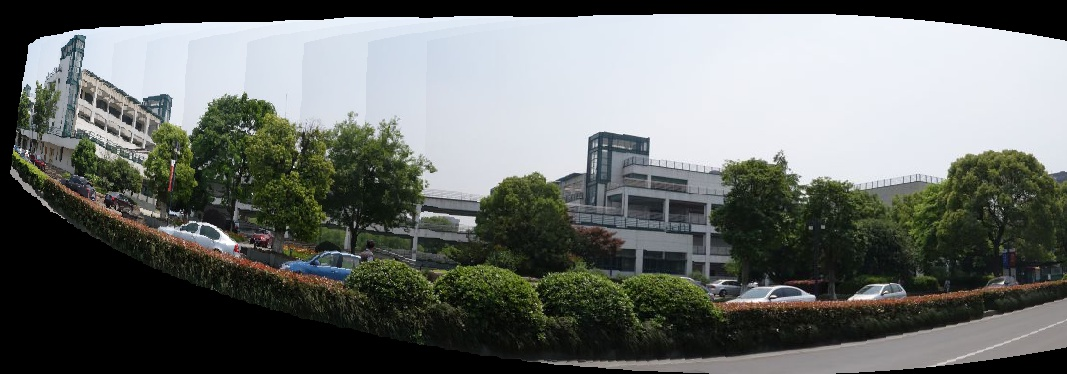
\includegraphics[width=0.65\textwidth]{output1} % Include the image placeholder.png
\caption{Panorama 1}
% 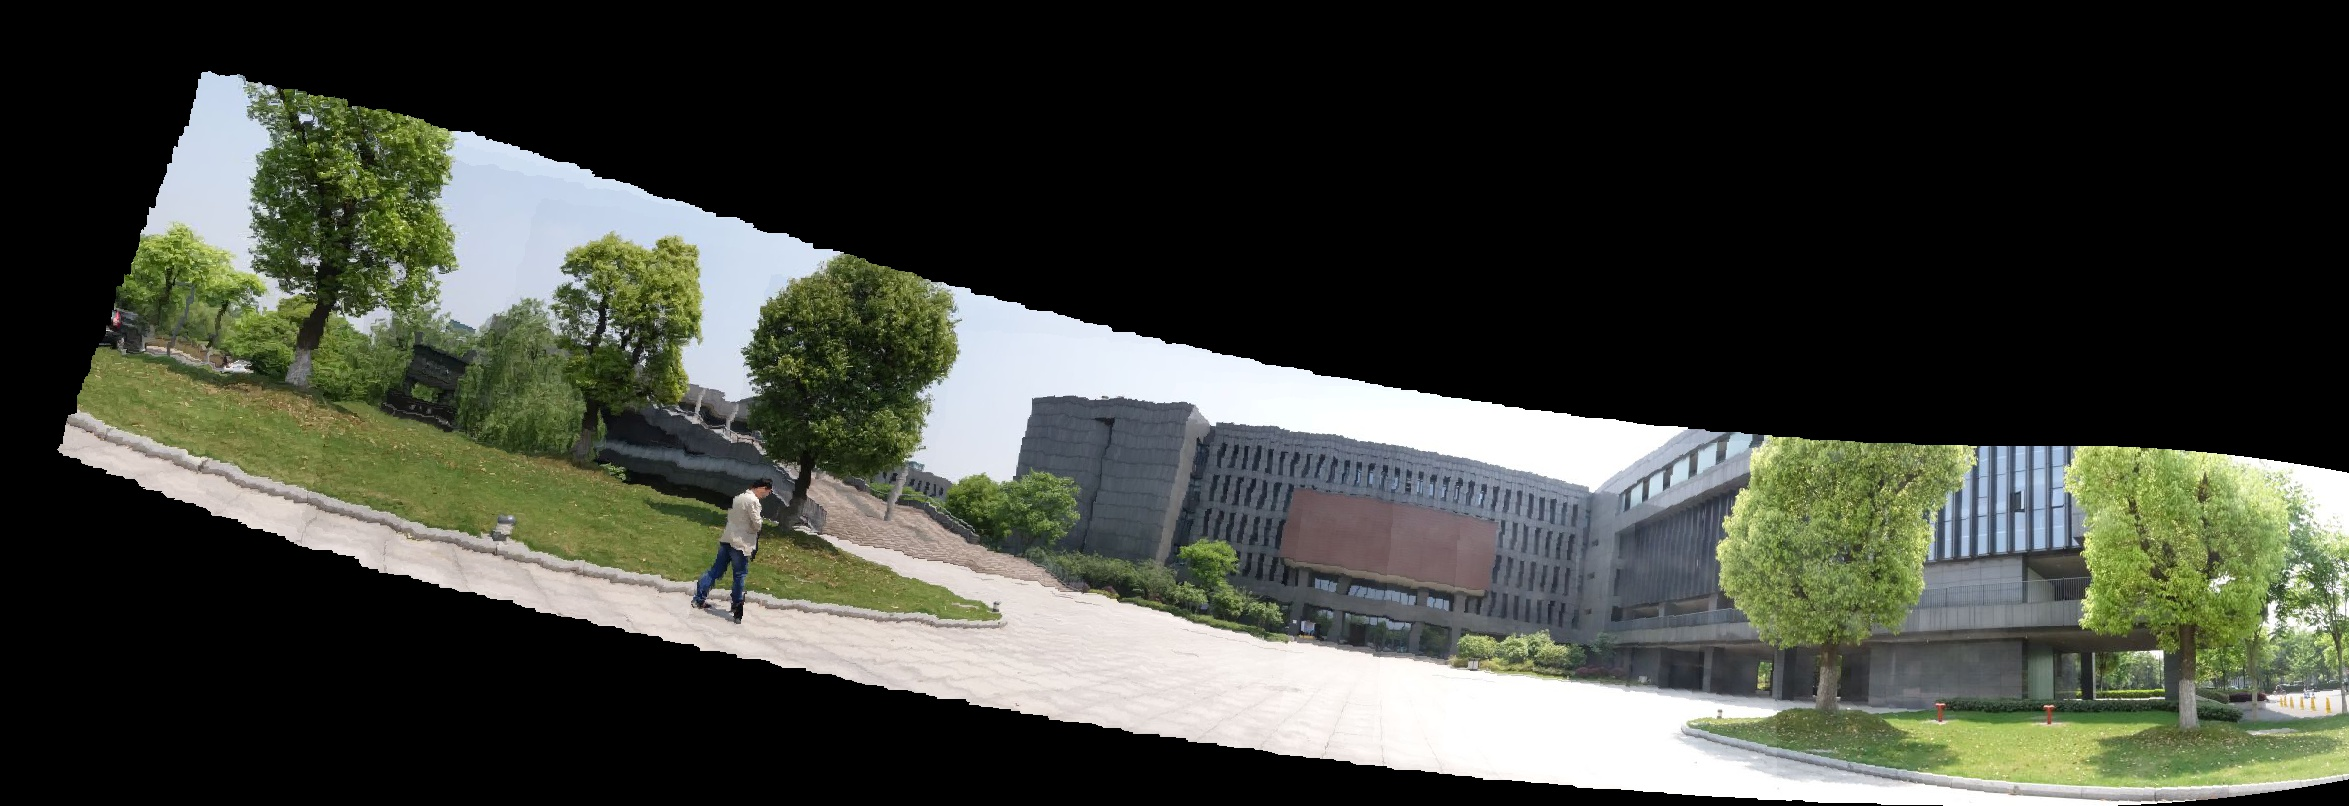
\includegraphics[width=0.65\textwidth]{output2} % Include the image placeholder.png
% \caption{Panorama 2}
\end{center}
\end{figure}

\begin{figure}[H]
\begin{center}
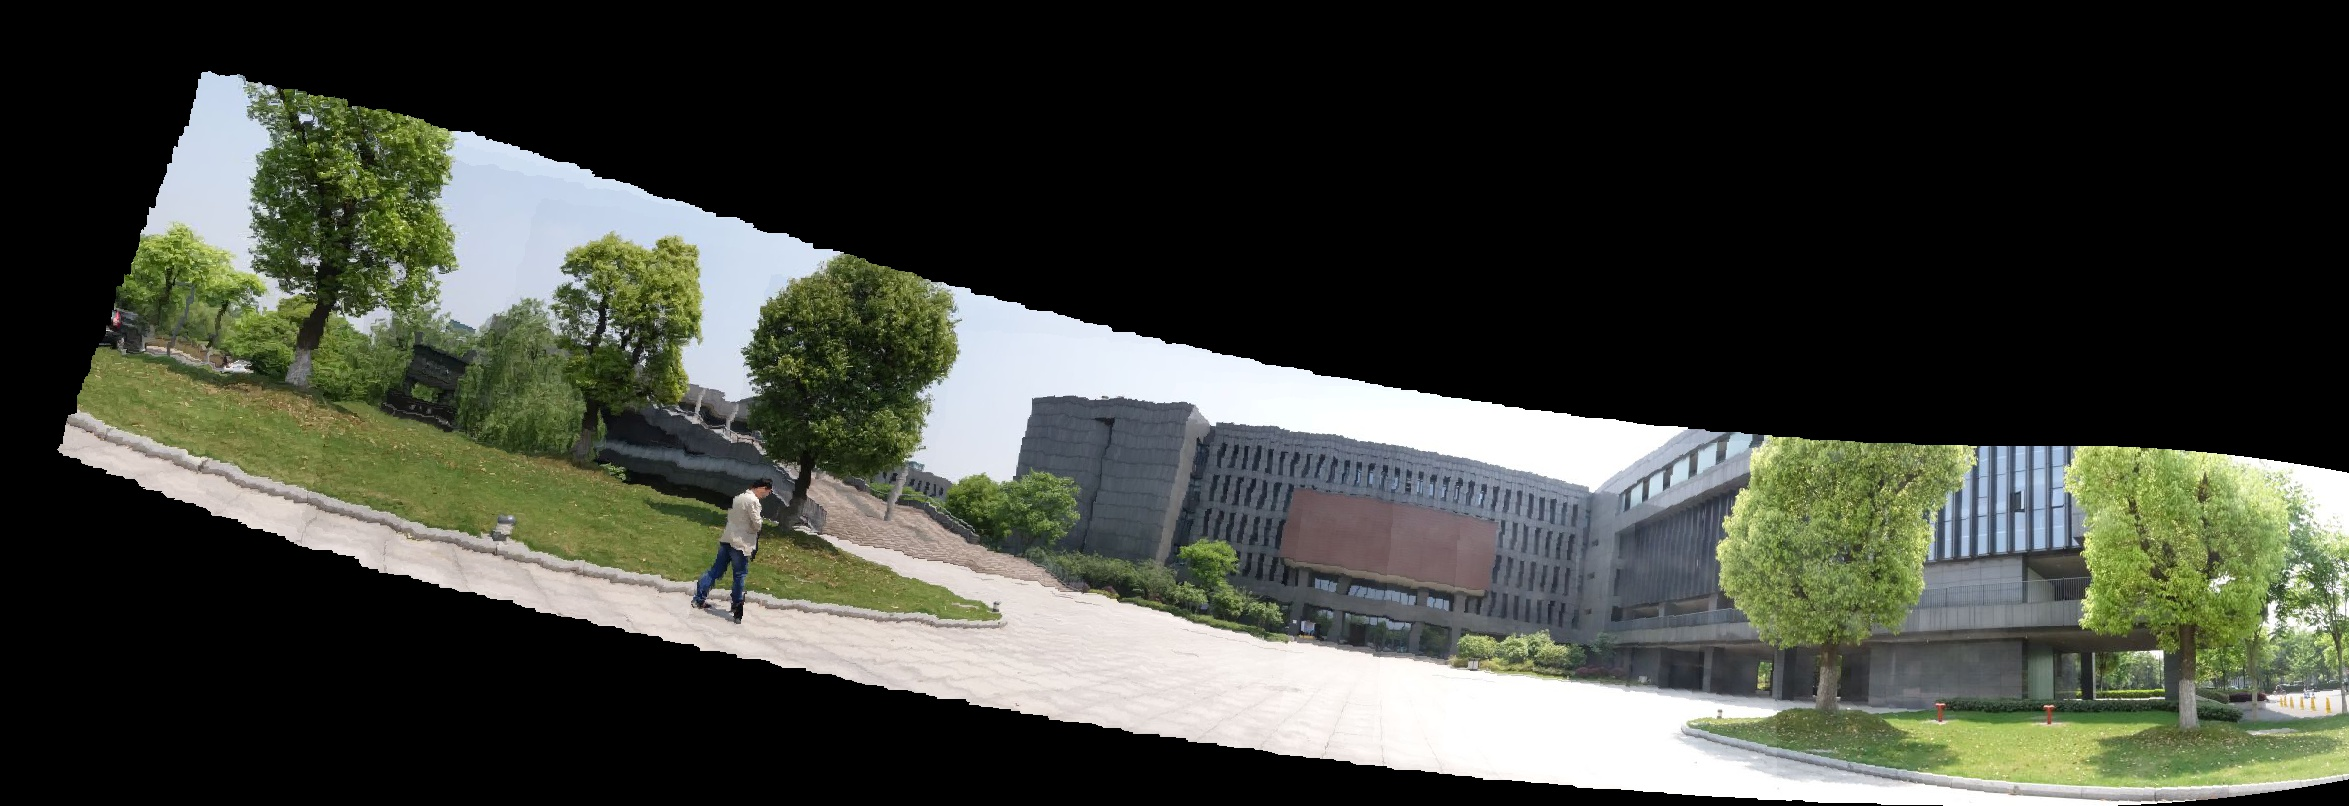
\includegraphics[width=0.65\textwidth]{output2} % Include the image placeholder.png
\caption{Panorama 2}
\end{center}
\end{figure}

%----------------------------------------------------------------------------------------
%	SECTION 5
%----------------------------------------------------------------------------------------

\section{实验心得}

% The accepted value (periodic table) is \SI{24.3}{\gram\per\mole} \cite{Smith:2012qr}. The percentage discrepancy between the accepted value and the result obtained here is 1.3\%. Because only a single measurement was made, it is not possible to calculate an estimated standard deviation.

% The most obvious source of experimental uncertainty is the limited precision of the balance. Other potential sources of experimental uncertainty are: the reaction might not be complete; if not enough time was allowed for total oxidation, less than complete oxidation of the magnesium might have, in part, reacted with nitrogen in the air (incorrect reaction); the magnesium oxide might have absorbed water from the air, and thus weigh ``too much." Because the result obtained is close to the accepted value it is possible that some of these experimental uncertainties have fortuitously cancelled one another.

本次实验实现了柱面全景拼接。整个流程中熟悉了OpenCV对于图像的处理,
SIFT特征点的提取和匹配,基于匹配点的变换的计算。




%----------------------------------------------------------------------------------------
%	SECTION 6
%----------------------------------------------------------------------------------------

% \section{Answers to Definitions}

% \begin{enumerate}
% \begin{item}
% The \emph{atomic weight of an element} is the relative weight of one of its atoms compared to C-12 with a weight of 12.0000000$\ldots$, hydrogen with a weight of 1.008, to oxygen with a weight of 16.00. Atomic weight is also the average weight of all the atoms of that element as they occur in nature.
% \end{item}
% \begin{item}
% The \emph{units of atomic weight} are two-fold, with an identical numerical value. They are g/mole of atoms (or just g/mol) or amu/atom.
% \end{item}
% \begin{item}
% \emph{Percentage discrepancy} between an accepted (literature) value and an experimental value is
% \begin{equation*}
% \frac{\mathrm{experimental\;result} - \mathrm{accepted\;result}}{\mathrm{accepted\;result}}
% \end{equation*}
% \end{item}
% \end{enumerate}

%----------------------------------------------------------------------------------------
%	BIBLIOGRAPHY
%----------------------------------------------------------------------------------------

% \bibliographystyle{apalike}

% \bibliography{sample}

%----------------------------------------------------------------------------------------


\end{document}